% Created by tikzDevice version 0.12.3.1 on 2021-12-14 20:04:36
% !TEX encoding = UTF-8 Unicode
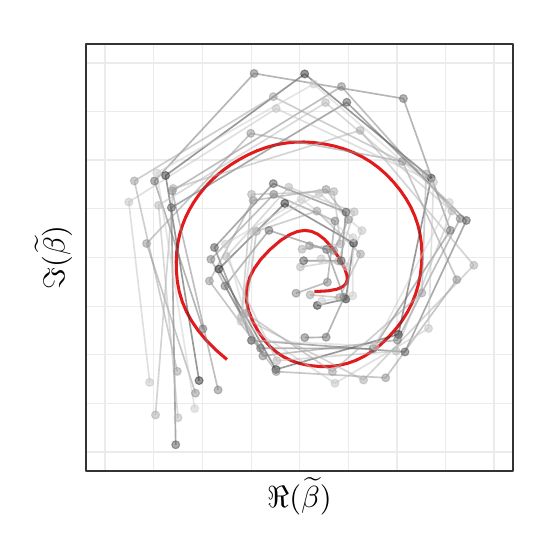
\begin{tikzpicture}[x=1pt,y=1pt]
\definecolor{fillColor}{RGB}{255,255,255}
\begin{scope}
\definecolor{drawColor}{RGB}{255,255,255}
\definecolor{fillColor}{RGB}{255,255,255}

\path[draw=drawColor,line width= 0.6pt,line join=round,line cap=round,fill=fillColor] (  0.00,  0.00) rectangle (180.67,180.68);
\end{scope}
\begin{scope}
\definecolor{fillColor}{RGB}{255,255,255}

\path[fill=fillColor] ( 20.71, 20.71) rectangle (175.17,175.17);
\definecolor{drawColor}{gray}{0.92}

\path[draw=drawColor,line width= 0.3pt,line join=round] ( 20.71, 45.29) --
	(175.17, 45.29);

\path[draw=drawColor,line width= 0.3pt,line join=round] ( 20.71, 80.39) --
	(175.17, 80.39);

\path[draw=drawColor,line width= 0.3pt,line join=round] ( 20.71,115.50) --
	(175.17,115.50);

\path[draw=drawColor,line width= 0.3pt,line join=round] ( 20.71,150.60) --
	(175.17,150.60);

\path[draw=drawColor,line width= 0.3pt,line join=round] ( 45.29, 20.71) --
	( 45.29,175.17);

\path[draw=drawColor,line width= 0.3pt,line join=round] ( 80.39, 20.71) --
	( 80.39,175.17);

\path[draw=drawColor,line width= 0.3pt,line join=round] (115.50, 20.71) --
	(115.50,175.17);

\path[draw=drawColor,line width= 0.3pt,line join=round] (150.60, 20.71) --
	(150.60,175.17);

\path[draw=drawColor,line width= 0.6pt,line join=round] ( 20.71, 27.74) --
	(175.17, 27.74);

\path[draw=drawColor,line width= 0.6pt,line join=round] ( 20.71, 62.84) --
	(175.17, 62.84);

\path[draw=drawColor,line width= 0.6pt,line join=round] ( 20.71, 97.94) --
	(175.17, 97.94);

\path[draw=drawColor,line width= 0.6pt,line join=round] ( 20.71,133.05) --
	(175.17,133.05);

\path[draw=drawColor,line width= 0.6pt,line join=round] ( 20.71,168.15) --
	(175.17,168.15);

\path[draw=drawColor,line width= 0.6pt,line join=round] ( 27.74, 20.71) --
	( 27.74,175.17);

\path[draw=drawColor,line width= 0.6pt,line join=round] ( 62.84, 20.71) --
	( 62.84,175.17);

\path[draw=drawColor,line width= 0.6pt,line join=round] ( 97.94, 20.71) --
	( 97.94,175.17);

\path[draw=drawColor,line width= 0.6pt,line join=round] (133.05, 20.71) --
	(133.05,175.17);

\path[draw=drawColor,line width= 0.6pt,line join=round] (168.15, 20.71) --
	(168.15,175.17);
\definecolor{drawColor}{RGB}{227,26,28}

\path[draw=drawColor,line width= 1.1pt,line join=round] (103.31, 85.62) --
	(108.31, 85.88) --
	(111.57, 86.51) --
	(113.53, 87.37) --
	(114.61, 88.38) --
	(115.12, 89.62) --
	(115.09, 91.32) --
	(114.33, 93.81) --
	(112.50, 97.36) --
	(109.63,101.57) --
	(106.92,104.54) --
	(104.45,106.40) --
	(102.12,107.41) --
	( 99.79,107.72) --
	( 97.29,107.36) --
	( 94.43,106.22) --
	( 91.07,104.08) --
	( 87.18,100.74) --
	( 83.94, 97.27) --
	( 81.60, 94.01) --
	( 80.00, 90.90) --
	( 79.05, 87.88) --
	( 78.67, 84.85) --
	( 78.85, 81.72) --
	( 79.63, 78.39) --
	( 81.09, 74.76) --
	( 83.00, 71.25) --
	( 85.05, 68.28) --
	( 87.25, 65.80) --
	( 89.61, 63.73) --
	( 92.17, 62.03) --
	( 94.97, 60.66) --
	( 98.06, 59.62) --
	(101.50, 58.90) --
	(105.20, 58.54) --
	(108.71, 58.55) --
	(112.02, 58.93) --
	(115.19, 59.66) --
	(118.25, 60.74) --
	(121.24, 62.20) --
	(124.20, 64.06) --
	(127.14, 66.37) --
	(130.08, 69.15) --
	(132.71, 72.09) --
	(134.98, 75.08) --
	(136.90, 78.16) --
	(138.51, 81.32) --
	(139.83, 84.61) --
	(140.85, 88.05) --
	(141.59, 91.67) --
	(142.04, 95.50) --
	(142.17, 99.34) --
	(141.97,102.97) --
	(141.47,106.44) --
	(140.67,109.78) --
	(139.55,113.02) --
	(138.12,116.18) --
	(136.35,119.29) --
	(134.21,122.38) --
	(131.75,125.37) --
	(129.17,128.04) --
	(126.48,130.40) --
	(123.66,132.47) --
	(120.69,134.27) --
	(117.56,135.81) --
	(114.24,137.11) --
	(110.69,138.16) --
	(106.92,138.95) --
	(103.20,139.46) --
	( 99.61,139.67) --
	( 96.11,139.60) --
	( 92.70,139.25) --
	( 89.34,138.63) --
	( 86.02,137.74) --
	( 82.71,136.55) --
	( 79.39,135.07) --
	( 76.20,133.36) --
	( 73.24,131.54) --
	( 70.52,129.60) --
	( 68.00,127.54) --
	( 65.67,125.34) --
	( 63.52,123.01) --
	( 61.54,120.53) --
	( 59.72,117.89) --
	( 58.08,115.10) --
	( 56.69,112.25) --
	( 55.55,109.33) --
	( 54.65,106.32) --
	( 53.99,103.20) --
	( 53.56, 99.95) --
	( 53.38, 96.55) --
	( 53.45, 92.96) --
	( 53.79, 89.20) --
	( 54.49, 85.50) --
	( 55.58, 81.93) --
	( 57.05, 78.43) --
	( 58.96, 74.98) --
	( 61.32, 71.53) --
	( 64.19, 68.08) --
	( 67.63, 64.59) --
	( 71.70, 61.06);
\definecolor{drawColor}{RGB}{51,51,51}

\path[draw=drawColor,draw opacity=0.50,line width= 0.6pt,line join=round] (104.34, 80.62) --
	(114.69, 82.93) --
	(117.44,103.10) --
	( 92.59,117.48) --
	( 68.76, 93.76) --
	( 89.40, 57.48) --
	(133.66, 70.14) --
	(145.54,126.61) --
	( 99.79,164.26) --
	( 49.55,127.55) --
	( 61.64, 53.46);
\definecolor{drawColor}{RGB}{87,87,87}

\path[draw=drawColor,draw opacity=0.50,line width= 0.6pt,line join=round] ( 99.44, 96.77) --
	(112.99, 96.77) --
	(114.73,114.33) --
	( 88.44,124.63) --
	( 67.19,101.55) --
	( 80.54, 67.98) --
	(136.02, 63.81) --
	(158.20,111.32) --
	(115.02,154.01) --
	( 51.63,115.95) --
	( 53.19, 30.27);
\definecolor{drawColor}{RGB}{110,110,110}

\path[draw=drawColor,draw opacity=0.50,line width= 0.6pt,line join=round] ( 99.83, 68.99) --
	(107.54, 69.13) --
	(114.03, 83.56) --
	(107.68,100.82) --
	( 86.90,107.74) --
	( 70.99, 87.64) --
	( 83.87, 65.16) --
	(124.51, 65.00) --
	(152.41,107.74) --
	(135.46,155.36) --
	( 81.52,164.44) --
	( 45.53,125.57) --
	( 63.01, 72.15);
\definecolor{drawColor}{RGB}{129,129,129}

\path[draw=drawColor,draw opacity=0.50,line width= 0.6pt,line join=round] ( 96.68, 85.02) --
	(107.98, 89.01) --
	(110.76,111.11) --
	( 88.62,120.76) --
	( 65.91, 97.29) --
	( 84.70, 62.38) --
	(133.28, 68.10) --
	(155.97,111.97) --
	(113.08,159.70) --
	( 51.91,121.99) --
	( 68.50, 50.07);
\definecolor{drawColor}{RGB}{145,145,145}

\path[draw=drawColor,draw opacity=0.50,line width= 0.6pt,line join=round] (101.53,102.21) --
	(110.31,100.44) --
	(115.65,111.67) --
	(107.52,122.52) --
	( 81.18,118.58) --
	( 65.38, 89.45) --
	( 89.51, 56.69) --
	(129.05, 54.47) --
	(154.76, 89.90) --
	(135.07,132.66) --
	( 80.32,142.79) --
	( 42.68,102.99) --
	( 60.33, 48.90);
\definecolor{drawColor}{RGB}{159,159,159}

\path[draw=drawColor,draw opacity=0.50,line width= 0.6pt,line join=round] (101.78, 84.44) --
	(112.39, 83.48) --
	(119.96, 99.18) --
	(104.20,114.69) --
	( 82.39,107.44) --
	( 78.50, 77.78) --
	(109.82, 56.69) --
	(142.15, 85.11) --
	(143.69,128.08) --
	( 88.45,156.04) --
	( 38.25,125.60) --
	( 53.76, 56.80);
\definecolor{drawColor}{RGB}{171,171,171}

\path[draw=drawColor,draw opacity=0.50,line width= 0.6pt,line join=round] ( 98.85,100.95) --
	(112.71,102.85) --
	(110.32,121.75) --
	( 80.59,120.74) --
	( 76.96, 76.56) --
	(121.06, 53.68) --
	(160.92, 95.14) --
	(119.85,143.86) --
	( 52.28,122.86) --
	( 45.89, 41.04);
\definecolor{drawColor}{RGB}{183,183,183}

\path[draw=drawColor,draw opacity=0.50,line width= 0.6pt,line join=round] ( 98.26, 94.52) --
	(111.98, 96.64) --
	(117.69,114.44) --
	( 94.04,123.31) --
	( 71.52, 98.28) --
	( 89.72, 60.64) --
	(132.84, 64.10) --
	(153.00,114.74) --
	(107.35,153.88) --
	( 46.98,116.81) --
	( 54.02, 40.04);
\definecolor{drawColor}{RGB}{194,194,194}

\path[draw=drawColor,draw opacity=0.50,line width= 0.6pt,line join=round] (105.73, 97.44) --
	(114.89, 94.68) --
	(120.49,107.66) --
	(105.09,121.11) --
	( 81.14,107.10) --
	( 76.81, 74.80) --
	(110.74, 52.50) --
	(144.56, 72.30) --
	(146.33,125.17) --
	( 89.51,151.77) --
	( 36.25,117.98) --
	( 43.79, 52.83);
\definecolor{drawColor}{RGB}{204,204,204}

\path[draw=drawColor,draw opacity=0.50,line width= 0.6pt,line join=round] (105.93, 82.12) --
	(117.17, 84.13) --
	(117.25,105.09) --
	( 98.53,119.04) --
	( 71.14,102.75) --
	( 80.76, 68.03) --
	(125.08, 65.93) --
	(152.07,117.84) --
	(103.04,160.61) --
	( 46.38,128.50) --
	( 60.04, 43.34);
\definecolor{drawColor}{RGB}{51,51,51}
\definecolor{fillColor}{RGB}{51,51,51}

\path[draw=drawColor,draw opacity=0.50,line width= 0.4pt,line join=round,line cap=round,fill=fillColor,fill opacity=0.50] (104.34, 80.62) circle (  1.43);

\path[draw=drawColor,draw opacity=0.50,line width= 0.4pt,line join=round,line cap=round,fill=fillColor,fill opacity=0.50] (114.69, 82.93) circle (  1.43);

\path[draw=drawColor,draw opacity=0.50,line width= 0.4pt,line join=round,line cap=round,fill=fillColor,fill opacity=0.50] (117.44,103.10) circle (  1.43);

\path[draw=drawColor,draw opacity=0.50,line width= 0.4pt,line join=round,line cap=round,fill=fillColor,fill opacity=0.50] ( 92.59,117.48) circle (  1.43);

\path[draw=drawColor,draw opacity=0.50,line width= 0.4pt,line join=round,line cap=round,fill=fillColor,fill opacity=0.50] ( 68.76, 93.76) circle (  1.43);

\path[draw=drawColor,draw opacity=0.50,line width= 0.4pt,line join=round,line cap=round,fill=fillColor,fill opacity=0.50] ( 89.40, 57.48) circle (  1.43);

\path[draw=drawColor,draw opacity=0.50,line width= 0.4pt,line join=round,line cap=round,fill=fillColor,fill opacity=0.50] (133.66, 70.14) circle (  1.43);

\path[draw=drawColor,draw opacity=0.50,line width= 0.4pt,line join=round,line cap=round,fill=fillColor,fill opacity=0.50] (145.54,126.61) circle (  1.43);

\path[draw=drawColor,draw opacity=0.50,line width= 0.4pt,line join=round,line cap=round,fill=fillColor,fill opacity=0.50] ( 99.79,164.26) circle (  1.43);

\path[draw=drawColor,draw opacity=0.50,line width= 0.4pt,line join=round,line cap=round,fill=fillColor,fill opacity=0.50] ( 49.55,127.55) circle (  1.43);

\path[draw=drawColor,draw opacity=0.50,line width= 0.4pt,line join=round,line cap=round,fill=fillColor,fill opacity=0.50] ( 61.64, 53.46) circle (  1.43);
\definecolor{drawColor}{RGB}{110,110,110}
\definecolor{fillColor}{RGB}{110,110,110}

\path[draw=drawColor,draw opacity=0.50,line width= 0.4pt,line join=round,line cap=round,fill=fillColor,fill opacity=0.50] ( 99.83, 68.99) circle (  1.43);

\path[draw=drawColor,draw opacity=0.50,line width= 0.4pt,line join=round,line cap=round,fill=fillColor,fill opacity=0.50] (107.54, 69.13) circle (  1.43);

\path[draw=drawColor,draw opacity=0.50,line width= 0.4pt,line join=round,line cap=round,fill=fillColor,fill opacity=0.50] (114.03, 83.56) circle (  1.43);

\path[draw=drawColor,draw opacity=0.50,line width= 0.4pt,line join=round,line cap=round,fill=fillColor,fill opacity=0.50] (107.68,100.82) circle (  1.43);

\path[draw=drawColor,draw opacity=0.50,line width= 0.4pt,line join=round,line cap=round,fill=fillColor,fill opacity=0.50] ( 86.90,107.74) circle (  1.43);

\path[draw=drawColor,draw opacity=0.50,line width= 0.4pt,line join=round,line cap=round,fill=fillColor,fill opacity=0.50] ( 70.99, 87.64) circle (  1.43);

\path[draw=drawColor,draw opacity=0.50,line width= 0.4pt,line join=round,line cap=round,fill=fillColor,fill opacity=0.50] ( 83.87, 65.16) circle (  1.43);

\path[draw=drawColor,draw opacity=0.50,line width= 0.4pt,line join=round,line cap=round,fill=fillColor,fill opacity=0.50] (124.51, 65.00) circle (  1.43);

\path[draw=drawColor,draw opacity=0.50,line width= 0.4pt,line join=round,line cap=round,fill=fillColor,fill opacity=0.50] (152.41,107.74) circle (  1.43);

\path[draw=drawColor,draw opacity=0.50,line width= 0.4pt,line join=round,line cap=round,fill=fillColor,fill opacity=0.50] (135.46,155.36) circle (  1.43);

\path[draw=drawColor,draw opacity=0.50,line width= 0.4pt,line join=round,line cap=round,fill=fillColor,fill opacity=0.50] ( 81.52,164.44) circle (  1.43);

\path[draw=drawColor,draw opacity=0.50,line width= 0.4pt,line join=round,line cap=round,fill=fillColor,fill opacity=0.50] ( 45.53,125.57) circle (  1.43);

\path[draw=drawColor,draw opacity=0.50,line width= 0.4pt,line join=round,line cap=round,fill=fillColor,fill opacity=0.50] ( 63.01, 72.15) circle (  1.43);
\definecolor{drawColor}{RGB}{129,129,129}
\definecolor{fillColor}{RGB}{129,129,129}

\path[draw=drawColor,draw opacity=0.50,line width= 0.4pt,line join=round,line cap=round,fill=fillColor,fill opacity=0.50] ( 96.68, 85.02) circle (  1.43);

\path[draw=drawColor,draw opacity=0.50,line width= 0.4pt,line join=round,line cap=round,fill=fillColor,fill opacity=0.50] (107.98, 89.01) circle (  1.43);

\path[draw=drawColor,draw opacity=0.50,line width= 0.4pt,line join=round,line cap=round,fill=fillColor,fill opacity=0.50] (110.76,111.11) circle (  1.43);

\path[draw=drawColor,draw opacity=0.50,line width= 0.4pt,line join=round,line cap=round,fill=fillColor,fill opacity=0.50] ( 88.62,120.76) circle (  1.43);

\path[draw=drawColor,draw opacity=0.50,line width= 0.4pt,line join=round,line cap=round,fill=fillColor,fill opacity=0.50] ( 65.91, 97.29) circle (  1.43);

\path[draw=drawColor,draw opacity=0.50,line width= 0.4pt,line join=round,line cap=round,fill=fillColor,fill opacity=0.50] ( 84.70, 62.38) circle (  1.43);

\path[draw=drawColor,draw opacity=0.50,line width= 0.4pt,line join=round,line cap=round,fill=fillColor,fill opacity=0.50] (133.28, 68.10) circle (  1.43);

\path[draw=drawColor,draw opacity=0.50,line width= 0.4pt,line join=round,line cap=round,fill=fillColor,fill opacity=0.50] (155.97,111.97) circle (  1.43);

\path[draw=drawColor,draw opacity=0.50,line width= 0.4pt,line join=round,line cap=round,fill=fillColor,fill opacity=0.50] (113.08,159.70) circle (  1.43);

\path[draw=drawColor,draw opacity=0.50,line width= 0.4pt,line join=round,line cap=round,fill=fillColor,fill opacity=0.50] ( 51.91,121.99) circle (  1.43);

\path[draw=drawColor,draw opacity=0.50,line width= 0.4pt,line join=round,line cap=round,fill=fillColor,fill opacity=0.50] ( 68.50, 50.07) circle (  1.43);
\definecolor{drawColor}{RGB}{145,145,145}
\definecolor{fillColor}{RGB}{145,145,145}

\path[draw=drawColor,draw opacity=0.50,line width= 0.4pt,line join=round,line cap=round,fill=fillColor,fill opacity=0.50] (101.53,102.21) circle (  1.43);

\path[draw=drawColor,draw opacity=0.50,line width= 0.4pt,line join=round,line cap=round,fill=fillColor,fill opacity=0.50] (110.31,100.44) circle (  1.43);

\path[draw=drawColor,draw opacity=0.50,line width= 0.4pt,line join=round,line cap=round,fill=fillColor,fill opacity=0.50] (115.65,111.67) circle (  1.43);

\path[draw=drawColor,draw opacity=0.50,line width= 0.4pt,line join=round,line cap=round,fill=fillColor,fill opacity=0.50] (107.52,122.52) circle (  1.43);

\path[draw=drawColor,draw opacity=0.50,line width= 0.4pt,line join=round,line cap=round,fill=fillColor,fill opacity=0.50] ( 81.18,118.58) circle (  1.43);

\path[draw=drawColor,draw opacity=0.50,line width= 0.4pt,line join=round,line cap=round,fill=fillColor,fill opacity=0.50] ( 65.38, 89.45) circle (  1.43);

\path[draw=drawColor,draw opacity=0.50,line width= 0.4pt,line join=round,line cap=round,fill=fillColor,fill opacity=0.50] ( 89.51, 56.69) circle (  1.43);

\path[draw=drawColor,draw opacity=0.50,line width= 0.4pt,line join=round,line cap=round,fill=fillColor,fill opacity=0.50] (129.05, 54.47) circle (  1.43);

\path[draw=drawColor,draw opacity=0.50,line width= 0.4pt,line join=round,line cap=round,fill=fillColor,fill opacity=0.50] (154.76, 89.90) circle (  1.43);

\path[draw=drawColor,draw opacity=0.50,line width= 0.4pt,line join=round,line cap=round,fill=fillColor,fill opacity=0.50] (135.07,132.66) circle (  1.43);

\path[draw=drawColor,draw opacity=0.50,line width= 0.4pt,line join=round,line cap=round,fill=fillColor,fill opacity=0.50] ( 80.32,142.79) circle (  1.43);

\path[draw=drawColor,draw opacity=0.50,line width= 0.4pt,line join=round,line cap=round,fill=fillColor,fill opacity=0.50] ( 42.68,102.99) circle (  1.43);

\path[draw=drawColor,draw opacity=0.50,line width= 0.4pt,line join=round,line cap=round,fill=fillColor,fill opacity=0.50] ( 60.33, 48.90) circle (  1.43);
\definecolor{drawColor}{RGB}{159,159,159}
\definecolor{fillColor}{RGB}{159,159,159}

\path[draw=drawColor,draw opacity=0.50,line width= 0.4pt,line join=round,line cap=round,fill=fillColor,fill opacity=0.50] (101.78, 84.44) circle (  1.43);

\path[draw=drawColor,draw opacity=0.50,line width= 0.4pt,line join=round,line cap=round,fill=fillColor,fill opacity=0.50] (112.39, 83.48) circle (  1.43);

\path[draw=drawColor,draw opacity=0.50,line width= 0.4pt,line join=round,line cap=round,fill=fillColor,fill opacity=0.50] (119.96, 99.18) circle (  1.43);

\path[draw=drawColor,draw opacity=0.50,line width= 0.4pt,line join=round,line cap=round,fill=fillColor,fill opacity=0.50] (104.20,114.69) circle (  1.43);

\path[draw=drawColor,draw opacity=0.50,line width= 0.4pt,line join=round,line cap=round,fill=fillColor,fill opacity=0.50] ( 82.39,107.44) circle (  1.43);

\path[draw=drawColor,draw opacity=0.50,line width= 0.4pt,line join=round,line cap=round,fill=fillColor,fill opacity=0.50] ( 78.50, 77.78) circle (  1.43);

\path[draw=drawColor,draw opacity=0.50,line width= 0.4pt,line join=round,line cap=round,fill=fillColor,fill opacity=0.50] (109.82, 56.69) circle (  1.43);

\path[draw=drawColor,draw opacity=0.50,line width= 0.4pt,line join=round,line cap=round,fill=fillColor,fill opacity=0.50] (142.15, 85.11) circle (  1.43);

\path[draw=drawColor,draw opacity=0.50,line width= 0.4pt,line join=round,line cap=round,fill=fillColor,fill opacity=0.50] (143.69,128.08) circle (  1.43);

\path[draw=drawColor,draw opacity=0.50,line width= 0.4pt,line join=round,line cap=round,fill=fillColor,fill opacity=0.50] ( 88.45,156.04) circle (  1.43);

\path[draw=drawColor,draw opacity=0.50,line width= 0.4pt,line join=round,line cap=round,fill=fillColor,fill opacity=0.50] ( 38.25,125.60) circle (  1.43);

\path[draw=drawColor,draw opacity=0.50,line width= 0.4pt,line join=round,line cap=round,fill=fillColor,fill opacity=0.50] ( 53.76, 56.80) circle (  1.43);
\definecolor{drawColor}{RGB}{171,171,171}
\definecolor{fillColor}{RGB}{171,171,171}

\path[draw=drawColor,draw opacity=0.50,line width= 0.4pt,line join=round,line cap=round,fill=fillColor,fill opacity=0.50] ( 98.85,100.95) circle (  1.43);

\path[draw=drawColor,draw opacity=0.50,line width= 0.4pt,line join=round,line cap=round,fill=fillColor,fill opacity=0.50] (112.71,102.85) circle (  1.43);

\path[draw=drawColor,draw opacity=0.50,line width= 0.4pt,line join=round,line cap=round,fill=fillColor,fill opacity=0.50] (110.32,121.75) circle (  1.43);

\path[draw=drawColor,draw opacity=0.50,line width= 0.4pt,line join=round,line cap=round,fill=fillColor,fill opacity=0.50] ( 80.59,120.74) circle (  1.43);

\path[draw=drawColor,draw opacity=0.50,line width= 0.4pt,line join=round,line cap=round,fill=fillColor,fill opacity=0.50] ( 76.96, 76.56) circle (  1.43);

\path[draw=drawColor,draw opacity=0.50,line width= 0.4pt,line join=round,line cap=round,fill=fillColor,fill opacity=0.50] (121.06, 53.68) circle (  1.43);

\path[draw=drawColor,draw opacity=0.50,line width= 0.4pt,line join=round,line cap=round,fill=fillColor,fill opacity=0.50] (160.92, 95.14) circle (  1.43);

\path[draw=drawColor,draw opacity=0.50,line width= 0.4pt,line join=round,line cap=round,fill=fillColor,fill opacity=0.50] (119.85,143.86) circle (  1.43);

\path[draw=drawColor,draw opacity=0.50,line width= 0.4pt,line join=round,line cap=round,fill=fillColor,fill opacity=0.50] ( 52.28,122.86) circle (  1.43);

\path[draw=drawColor,draw opacity=0.50,line width= 0.4pt,line join=round,line cap=round,fill=fillColor,fill opacity=0.50] ( 45.89, 41.04) circle (  1.43);
\definecolor{drawColor}{RGB}{183,183,183}
\definecolor{fillColor}{RGB}{183,183,183}

\path[draw=drawColor,draw opacity=0.50,line width= 0.4pt,line join=round,line cap=round,fill=fillColor,fill opacity=0.50] ( 98.26, 94.52) circle (  1.43);

\path[draw=drawColor,draw opacity=0.50,line width= 0.4pt,line join=round,line cap=round,fill=fillColor,fill opacity=0.50] (111.98, 96.64) circle (  1.43);

\path[draw=drawColor,draw opacity=0.50,line width= 0.4pt,line join=round,line cap=round,fill=fillColor,fill opacity=0.50] (117.69,114.44) circle (  1.43);

\path[draw=drawColor,draw opacity=0.50,line width= 0.4pt,line join=round,line cap=round,fill=fillColor,fill opacity=0.50] ( 94.04,123.31) circle (  1.43);

\path[draw=drawColor,draw opacity=0.50,line width= 0.4pt,line join=round,line cap=round,fill=fillColor,fill opacity=0.50] ( 71.52, 98.28) circle (  1.43);

\path[draw=drawColor,draw opacity=0.50,line width= 0.4pt,line join=round,line cap=round,fill=fillColor,fill opacity=0.50] ( 89.72, 60.64) circle (  1.43);

\path[draw=drawColor,draw opacity=0.50,line width= 0.4pt,line join=round,line cap=round,fill=fillColor,fill opacity=0.50] (132.84, 64.10) circle (  1.43);

\path[draw=drawColor,draw opacity=0.50,line width= 0.4pt,line join=round,line cap=round,fill=fillColor,fill opacity=0.50] (153.00,114.74) circle (  1.43);

\path[draw=drawColor,draw opacity=0.50,line width= 0.4pt,line join=round,line cap=round,fill=fillColor,fill opacity=0.50] (107.35,153.88) circle (  1.43);

\path[draw=drawColor,draw opacity=0.50,line width= 0.4pt,line join=round,line cap=round,fill=fillColor,fill opacity=0.50] ( 46.98,116.81) circle (  1.43);

\path[draw=drawColor,draw opacity=0.50,line width= 0.4pt,line join=round,line cap=round,fill=fillColor,fill opacity=0.50] ( 54.02, 40.04) circle (  1.43);
\definecolor{drawColor}{RGB}{194,194,194}
\definecolor{fillColor}{RGB}{194,194,194}

\path[draw=drawColor,draw opacity=0.50,line width= 0.4pt,line join=round,line cap=round,fill=fillColor,fill opacity=0.50] (105.73, 97.44) circle (  1.43);

\path[draw=drawColor,draw opacity=0.50,line width= 0.4pt,line join=round,line cap=round,fill=fillColor,fill opacity=0.50] (114.89, 94.68) circle (  1.43);

\path[draw=drawColor,draw opacity=0.50,line width= 0.4pt,line join=round,line cap=round,fill=fillColor,fill opacity=0.50] (120.49,107.66) circle (  1.43);

\path[draw=drawColor,draw opacity=0.50,line width= 0.4pt,line join=round,line cap=round,fill=fillColor,fill opacity=0.50] (105.09,121.11) circle (  1.43);

\path[draw=drawColor,draw opacity=0.50,line width= 0.4pt,line join=round,line cap=round,fill=fillColor,fill opacity=0.50] ( 81.14,107.10) circle (  1.43);

\path[draw=drawColor,draw opacity=0.50,line width= 0.4pt,line join=round,line cap=round,fill=fillColor,fill opacity=0.50] ( 76.81, 74.80) circle (  1.43);

\path[draw=drawColor,draw opacity=0.50,line width= 0.4pt,line join=round,line cap=round,fill=fillColor,fill opacity=0.50] (110.74, 52.50) circle (  1.43);

\path[draw=drawColor,draw opacity=0.50,line width= 0.4pt,line join=round,line cap=round,fill=fillColor,fill opacity=0.50] (144.56, 72.30) circle (  1.43);

\path[draw=drawColor,draw opacity=0.50,line width= 0.4pt,line join=round,line cap=round,fill=fillColor,fill opacity=0.50] (146.33,125.17) circle (  1.43);

\path[draw=drawColor,draw opacity=0.50,line width= 0.4pt,line join=round,line cap=round,fill=fillColor,fill opacity=0.50] ( 89.51,151.77) circle (  1.43);

\path[draw=drawColor,draw opacity=0.50,line width= 0.4pt,line join=round,line cap=round,fill=fillColor,fill opacity=0.50] ( 36.25,117.98) circle (  1.43);

\path[draw=drawColor,draw opacity=0.50,line width= 0.4pt,line join=round,line cap=round,fill=fillColor,fill opacity=0.50] ( 43.79, 52.83) circle (  1.43);
\definecolor{drawColor}{RGB}{204,204,204}
\definecolor{fillColor}{RGB}{204,204,204}

\path[draw=drawColor,draw opacity=0.50,line width= 0.4pt,line join=round,line cap=round,fill=fillColor,fill opacity=0.50] (105.93, 82.12) circle (  1.43);

\path[draw=drawColor,draw opacity=0.50,line width= 0.4pt,line join=round,line cap=round,fill=fillColor,fill opacity=0.50] (117.17, 84.13) circle (  1.43);

\path[draw=drawColor,draw opacity=0.50,line width= 0.4pt,line join=round,line cap=round,fill=fillColor,fill opacity=0.50] (117.25,105.09) circle (  1.43);

\path[draw=drawColor,draw opacity=0.50,line width= 0.4pt,line join=round,line cap=round,fill=fillColor,fill opacity=0.50] ( 98.53,119.04) circle (  1.43);

\path[draw=drawColor,draw opacity=0.50,line width= 0.4pt,line join=round,line cap=round,fill=fillColor,fill opacity=0.50] ( 71.14,102.75) circle (  1.43);

\path[draw=drawColor,draw opacity=0.50,line width= 0.4pt,line join=round,line cap=round,fill=fillColor,fill opacity=0.50] ( 80.76, 68.03) circle (  1.43);

\path[draw=drawColor,draw opacity=0.50,line width= 0.4pt,line join=round,line cap=round,fill=fillColor,fill opacity=0.50] (125.08, 65.93) circle (  1.43);

\path[draw=drawColor,draw opacity=0.50,line width= 0.4pt,line join=round,line cap=round,fill=fillColor,fill opacity=0.50] (152.07,117.84) circle (  1.43);

\path[draw=drawColor,draw opacity=0.50,line width= 0.4pt,line join=round,line cap=round,fill=fillColor,fill opacity=0.50] (103.04,160.61) circle (  1.43);

\path[draw=drawColor,draw opacity=0.50,line width= 0.4pt,line join=round,line cap=round,fill=fillColor,fill opacity=0.50] ( 46.38,128.50) circle (  1.43);

\path[draw=drawColor,draw opacity=0.50,line width= 0.4pt,line join=round,line cap=round,fill=fillColor,fill opacity=0.50] ( 60.04, 43.34) circle (  1.43);
\definecolor{drawColor}{RGB}{87,87,87}
\definecolor{fillColor}{RGB}{87,87,87}

\path[draw=drawColor,draw opacity=0.50,line width= 0.4pt,line join=round,line cap=round,fill=fillColor,fill opacity=0.50] ( 99.44, 96.77) circle (  1.43);

\path[draw=drawColor,draw opacity=0.50,line width= 0.4pt,line join=round,line cap=round,fill=fillColor,fill opacity=0.50] (112.99, 96.77) circle (  1.43);

\path[draw=drawColor,draw opacity=0.50,line width= 0.4pt,line join=round,line cap=round,fill=fillColor,fill opacity=0.50] (114.73,114.33) circle (  1.43);

\path[draw=drawColor,draw opacity=0.50,line width= 0.4pt,line join=round,line cap=round,fill=fillColor,fill opacity=0.50] ( 88.44,124.63) circle (  1.43);

\path[draw=drawColor,draw opacity=0.50,line width= 0.4pt,line join=round,line cap=round,fill=fillColor,fill opacity=0.50] ( 67.19,101.55) circle (  1.43);

\path[draw=drawColor,draw opacity=0.50,line width= 0.4pt,line join=round,line cap=round,fill=fillColor,fill opacity=0.50] ( 80.54, 67.98) circle (  1.43);

\path[draw=drawColor,draw opacity=0.50,line width= 0.4pt,line join=round,line cap=round,fill=fillColor,fill opacity=0.50] (136.02, 63.81) circle (  1.43);

\path[draw=drawColor,draw opacity=0.50,line width= 0.4pt,line join=round,line cap=round,fill=fillColor,fill opacity=0.50] (158.20,111.32) circle (  1.43);

\path[draw=drawColor,draw opacity=0.50,line width= 0.4pt,line join=round,line cap=round,fill=fillColor,fill opacity=0.50] (115.02,154.01) circle (  1.43);

\path[draw=drawColor,draw opacity=0.50,line width= 0.4pt,line join=round,line cap=round,fill=fillColor,fill opacity=0.50] ( 51.63,115.95) circle (  1.43);

\path[draw=drawColor,draw opacity=0.50,line width= 0.4pt,line join=round,line cap=round,fill=fillColor,fill opacity=0.50] ( 53.19, 30.27) circle (  1.43);
\definecolor{drawColor}{gray}{0.20}

\path[draw=drawColor,line width= 0.6pt,line join=round,line cap=round] ( 20.71, 20.71) rectangle (175.17,175.17);
\end{scope}
\begin{scope}
\definecolor{drawColor}{RGB}{0,0,0}

\node[text=drawColor,anchor=base,inner sep=0pt, outer sep=0pt, scale=  1.10] at ( 97.94,  7.64) {$\Re(\widetilde\beta)$};
\end{scope}
\begin{scope}
\definecolor{drawColor}{RGB}{0,0,0}

\node[text=drawColor,rotate= 90.00,anchor=base,inner sep=0pt, outer sep=0pt, scale=  1.10] at ( 13.08, 97.94) {$\Im(\widetilde\beta)$};
\end{scope}
\end{tikzpicture}
